\chapter{IIR Lookahead}
\label{chap:iir_lookahead}

In this chapter we will explain how we have improved the original IIR design by applying the techniques studied in the course,
specifically the lookahead, the pipelining and retiming. We derived the new architecture from the block diagram shown in
figure \ref{fig:iir}, then we have modified the C model to obtain a reference implementation and, finally, we have derived
the VHDL implementation to reproduce all the steps done in chapter \ref{chap:iir}. Hence, for this last part, we will
outline only the results and compare them to the IIR's one since the procedures we have followed are the same.

\section{Architecture derivation}

First, as mandated by exercise 2.4, we have applied the J-lookahead method with $J = 1$. This is a non-universal technique,
that is normally applied when other techniques such as pipelining, retiming, unfolding, ecc. cannot be applied. In our baseline
architecture there is actually space for universal techniques, as demonstrated below, although we have applied the lookahead
first nevertheless to comply with the exercise's request.

\subsection{Baseline IIR analysis}

\begin{figure}[!ht]
	\centering
	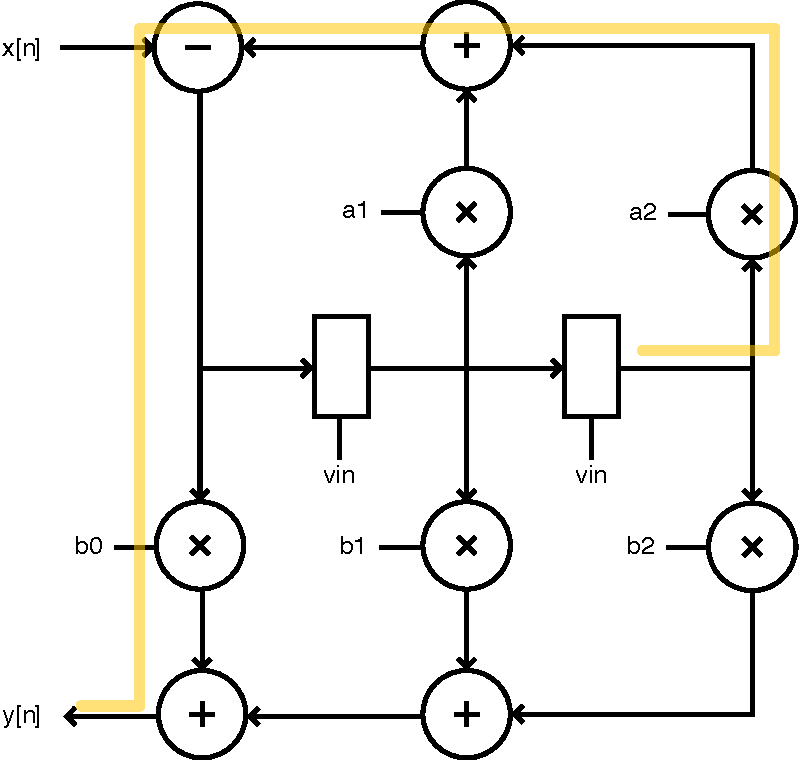
\includegraphics[width=0.4\linewidth]{./chapters/pictures/loop_bound_iir.pdf}
	\caption{Baseline IIR critical path}
	\label{fig:loop_bound_iir}
\end{figure}

In figure \ref{fig:loop_bound_iir} it is outlined in yellow the critical path of the non-optimized filter. If we define with
$T_{a}$ the delay of the adder and with with $T_{m}$ the delay of the multiplier, we obtain that

\begin{equation}
    \label{eq:baseline_iir_delay}
    CP_{iir} = 2T_{m} + 3T_{a}
\end{equation}

It can be also seen in the picture that there are two loops, namely $LB_{1}$ and $LB_{2}$. It is possible to calculate the
loop bound as follows:

\begin{align}
    LB_{iir_{1}} &= \frac{T_{m} + 2T_{a}}{1} \\
    LB_{iir_{2}} &= \frac{T_{m} + 2T_{a}}{2}
\end{align}

Hence, we obtain

\begin{equation}
    T_{iir_{\infty}} = \max \lbrace LB_{iir_{1}}, LB_{iir_{2}} \rbrace = LB_{iir_{1}} < CP_{iir}
\end{equation}

This means that a universal technique to improve the architecture exists; indeed pipelining could speed-up the architecture,
as there is a feed-forward cutset which divides the feed-forward multipliers from the upper part of the circuit. By placing
pipeline register there we obtain

\begin{equation}
    CP_{iir_{pipeline}} = T_{iir_{\infty}} = T_{m} + 2T_{a}
\end{equation}

This demonstrate that multiple optimization paths do exists for our architecture.

\subsection{Lookahead application}

The lookahead method works by recursively expanding the base equation. As the exercise stated that only one expansion was required,
we have proceeded in this way:

The equation of our filter is

\begin{equation}
    \label{eq:iir_eq}
    \begin{split}
        y[n] &= {\sum_{k=0}^{2} a_{k}y[n-k]} + {\sum_{i=0}^{2} b_{i}x[n-i]} = \\
        &= a_{0}y[n] + a_{1}y[n-1] + a_{2}y[n-2] + b_{0}x[n] + b_{1}x[n-1] + b_2[x-2]
    \end{split}
\end{equation}

We have calculated the formula of $y[n-1]$, which is

\begin{equation}
    \label{eq:yn-1}
    y[n-1] = a_{0}y[n-1] + a_{1}y[n-2] + a_{2}y[n-3] + b_{0}x[n-1] + b_{1}x[n-2] + b_2[x-3]
\end{equation}

If we insert \ref{eq:yn-1} in \ref{eq:iir_eq} the result is

\begin{equation}
    \label{eq:lookahead}
    \begin{split}
        y[n] &= a_{0}y[n] + a_{1}a_{0}y[n-1] + a^2_{1}y[n-2] + a_{1}a_{2}y[n-3] + a_{1}b_{0}x[n-1] + a_{1}b_{1}x[n-2]\ + \\
    & + a_{1}b_{2}x[n-3] + a_{2}y[n-2] + b_{0}x[n] + b_{1}x[n-1] + b_{2}x[n-2]
    \end{split}
\end{equation}

Which is our new filter's equation. Its block diagram is shown in figure \ref{fig:iir_lookahead}.

\begin{figure}[!ht]
	\centering
	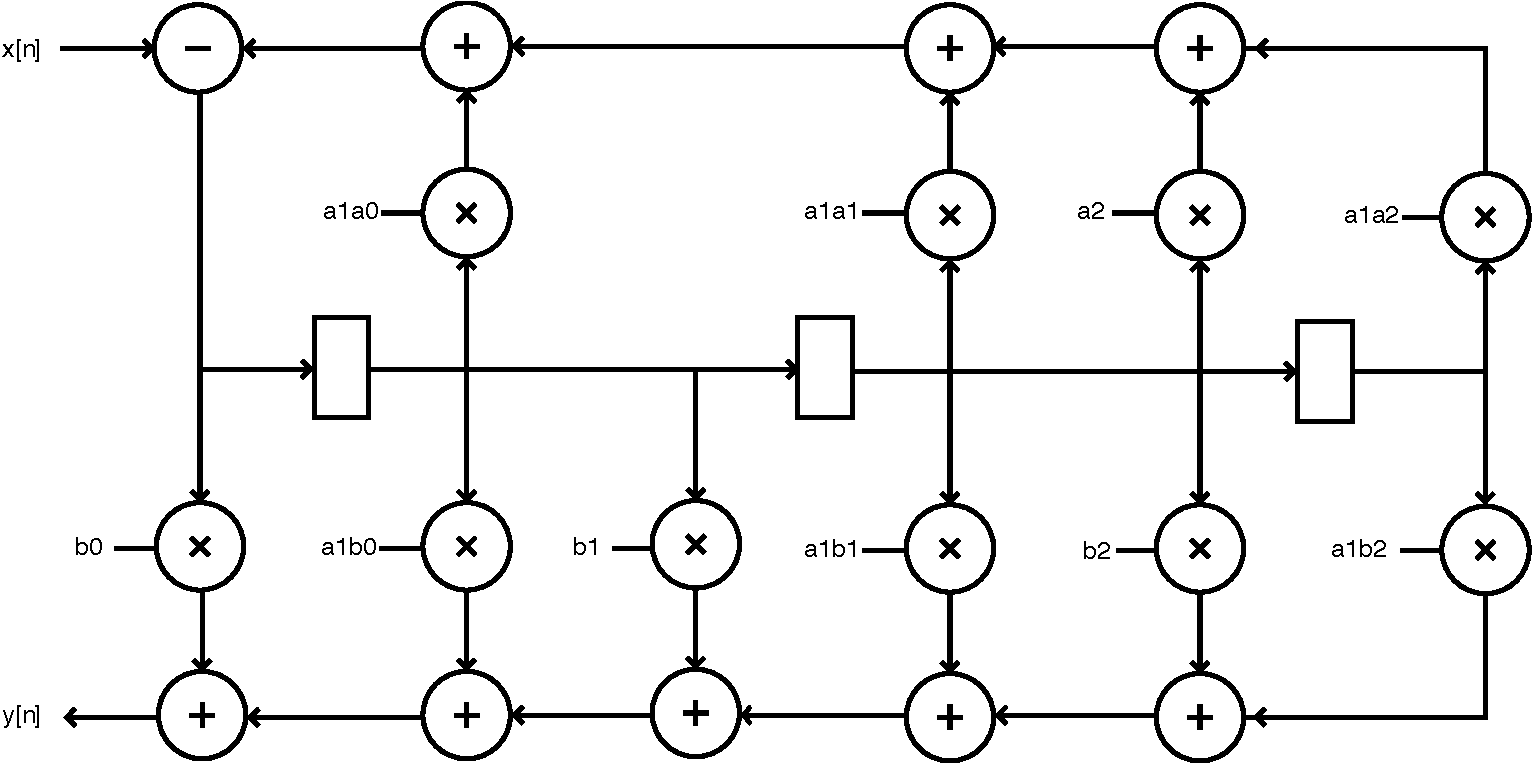
\includegraphics[width=0.7\linewidth]{./chapters/pictures/irr_lookahead.pdf}
	\caption{IIR lookahead}
	\label{fig:iir_lookahead}
\end{figure}

In equation \ref{eq:lookahead} it can be noticed that new coefficients appear in the form $a_{1}*a_{j}$ and $a_{1}*b_{j}$.
Their result does not fit in 12 bits, therefore we have decided to truncate them (by taking the 12 MSBs) to respect the original interface's bit width.

Starting from the structure shown in figure \ref{fig:iir_lookahead} we have derived a new C and VHDL model: the latter has been used as basis for the
optimizations described in section \ref{sec:iir_opt}, the former as golden model to check the results since, due to the new coefficients, the filter
has a different $THD$ and produces slightly different values. 

\section{Lookahead optimizations}
\label{sec:iir_opt}



\section{Results comparison}